\section{Environment Description}
\label{cha:env_description}

\subsection{Environment Simulation}
\label{sec:env_simulation}

The environment is simulated in the Unity game engine. The reinforcement learning algorithm is implemented in Python and builds upon the stable-baselines3 library. This library is able to train a proximal policy algorithm on any environment that implement the Gymnasium API. The Unity environment is wrapped in a Python class that implements the Gymnasium API. This class is responsible for the communication between the reinforcement learning algorithm and the Unity engine. The communication is implemented using \acs{RPC} with the Peaceful Pie \textcite{peacefulpie} library.

The interaction is shown in \ref{fig:communication_python_unity}.

\newcommand{\arenaImg}[1]{\includegraphics[width=0.15\textwidth]{Bilder/image_printer_images/agent_interaction/step_#1_arena.png}}
\newcommand{\agentImg}[1]{\includegraphics[width=0.15\textwidth]{Bilder/image_printer_images/agent_interaction/step_#1_image_from_unity.png}}

\newcommand\yOffsetc{-6.5}
\newcommand\xOffsetc{4.5}
\newcommand\envWidth{12}

\usetikzlibrary{decorations.pathreplacing}

\usetikzlibrary{fit}
\begin{figure}[h]
    \centering
    \begin{tikzpicture}[%
            every node/.style={
                    font=\scriptsize,
                    % Better alignment, see https://tex.stackexchange.com/questions/315075
                    text height=1ex,
                    text depth=.25ex,
                },
        ]

        \node[fit={(0,0) (0 + \envWidth, - 5)}, inner sep=0pt, draw=blue, thick] (env) {};
        \node[above] (envText) at (env.north) {Environment};
        \node[below] (envU) at (env.south) {Unity};

        \node[above] (oldState) at (2, -2)
        {\arenaImg{0}};
        \node[right] at (oldState.east) {old state};

        \node[below] (newState) at (2, -4)
        {\arenaImg{1}};
        \node[right] at (newState.east) {new state};


        \node[above] (oldImg) at (7, -2)
        {\agentImg{0}};
        \node[right] at (oldImg.east) {old agent camera image};

        \node[below] (newImg) at (7, -4)
        {\agentImg{1}};
        \node[right] at (newImg.east) {new agent camera image};
        
        
        \draw[->,thick] (2, -2)--(2, -3);
        \node[right] at (2, -2.5) {step (action / agent movement)};

        \draw[->,thick] (7, -2)--(7, -3);
        \node[right] at (7, -2.5) {step (action / agent movement)};


        % bottom half:
        \node[fit={(0 + \xOffsetc,0+ \yOffsetc) (3+ \xOffsetc,-1 + \yOffsetc)}, inner sep=0pt, fill=cyan, draw=blue, thick] (gym) {};
        \node[above] at (gym.north) {Python Gymnasium Environment};
        %\node[below] at (gym.south) {Python};


        % arrows communication
        \draw[->,thick, red] (\xOffsetc + 3, -0.5+ \yOffsetc)--(\envWidth+0.5, -0.5+\yOffsetc)--(\envWidth + 0.5, -2.5)--(\envWidth, -2.5);
        \node[below] at (\xOffsetc + 8, -0.5+ \yOffsetc) {reset and step commands};

        \draw[->,thick, red] (0, -2.5)--(-0.5,-2.5)--(-0.5,-0.5+\yOffsetc)--(\xOffsetc, -0.5+ \yOffsetc);
        \node[right] (camArrow) at (\xOffsetc -5, -0.5+ \yOffsetc) {\agentImg{1}};
        \node[below] at (camArrow.south) {rewards + new agent camera images};

        % arrow API
        \draw[<-,thick] (\xOffsetc + 1.5, -1 + \yOffsetc)--(\xOffsetc + 1.5,\yOffsetc - 3);
        \node[right] at (\xOffsetc + 1.5, \yOffsetc - 2) {Gymnasium API calls};

        % algos block
        \node[fit={(0 + \xOffsetc,0+ \yOffsetc -3) (3+ \xOffsetc,-1 + \yOffsetc -3)}, inner sep=0pt, fill=cyan, draw=blue, thick] (algo) {};
        \node[above] at (algo.north) {\acs{PPO} training and evaluation algorithms};
        \node[below] at (algo.south) {Python};

    \end{tikzpicture}
    \begin{tabular}{r@{: }l}
        red & RPC calls and returns \\
    \end{tabular}
    \caption{Communication between Python and Unity}
    \label{fig:communication_python_unity}
\end{figure}


\paragraph{Parallel environment procesing}

The stable-baselines3 library supports the parallel processing of multiple environments. The config parameter $n_envs$ specifies how many environments are simulated in parallel. The environments are simulated in the same Unity instance, see \ref{fig:parallel_simulation_unity_instance}. The seperation between the Unity engine and the Python algorithm requires \acs{RPC} calls for every environment step and reset. This can slow the training process. The overhead of sending calls to the Unity engine is reduced by bundling the calls for all environments in one \acs{RPC} call. The $use\_bundled\_calls$ config parameter enables the bundling of calls.

\begin{figure}
    \centering
    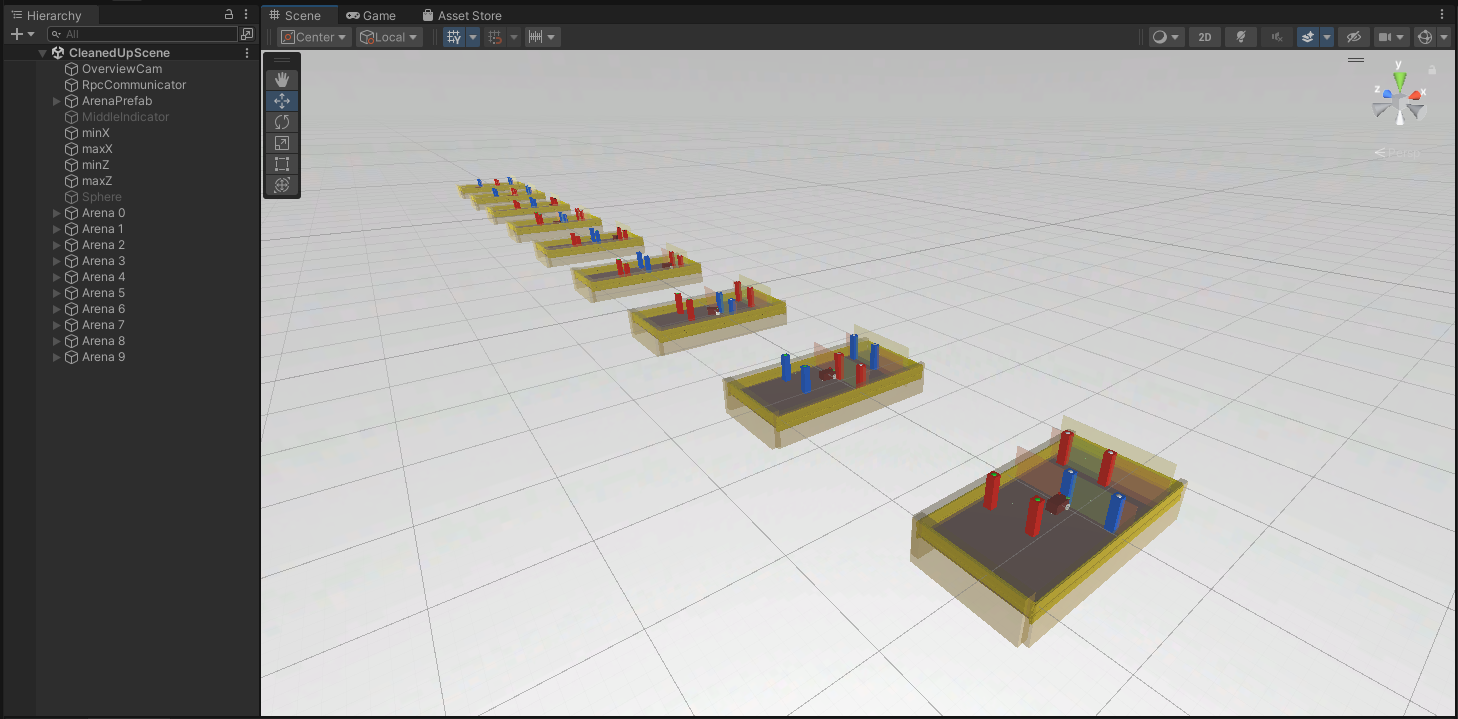
\includegraphics[width=0.8\textwidth]{Bilder/parallel_simulation_unity_instance.png}
    \caption{Parallel simulation of multiple environments in one Unity instance}
    \label{fig:parallel_simulation_unity_instance}
\end{figure}


\paragraph{Environment steps}
\label{sec:non_blocking_step_calls}

The step function of the Unity environment is non-blocking. This means that Unity returns the call before the entire step transition is complete. The python algorithm can continue without waiting for the step to complete. This interaction is shown in \ref{fig:step_call_timeline}.

In conventional reinforcement learning each step transition results in a new observation that is used to predict the next action. Since the Unity environment returns the call before the current step is finished, this is not possible. In this implementation the step call to Unity returns the observation from the start of the step instead. This observation does not capture the changes that have occurred in the environment during the step transition. The full changes are then visible to the agent after the next step has completed. 

\definecolor{myLightGray}{RGB}{191,191,191}
\definecolor{myDarkGray}{RGB}{144,144,144}
\definecolor{myBlue}{RGB}{0,191,255}


\newcommand\po{-3}

\newcommand\fo{-5}

\begin{figure}[h]
    \centering
    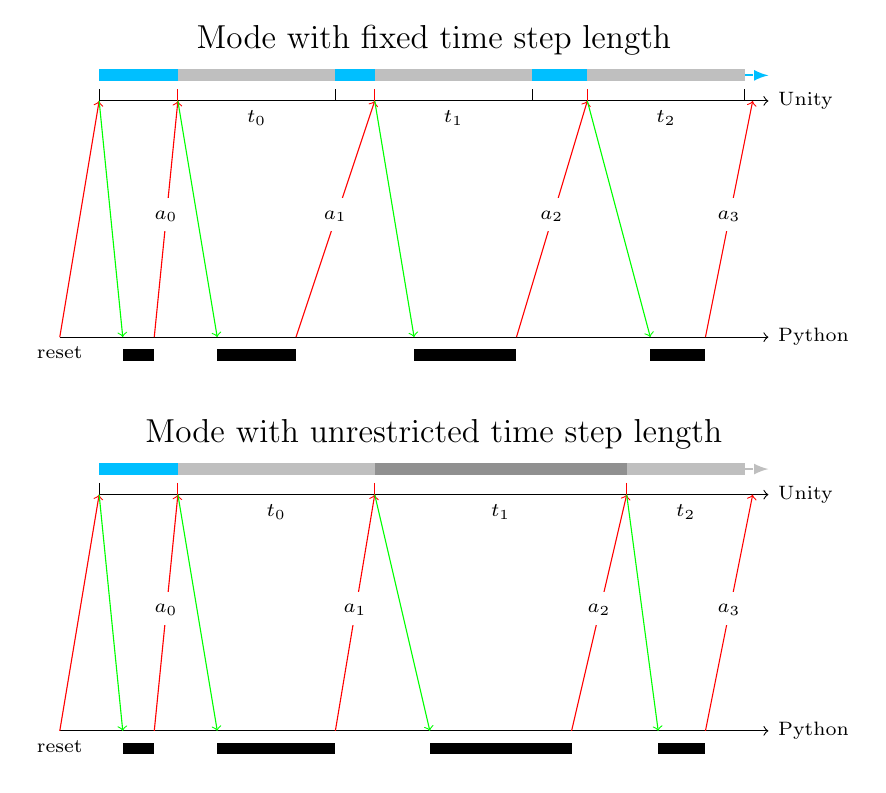
\begin{tikzpicture}[%
            every node/.style={
                    font=\scriptsize,
                    % Better alignment, see https://tex.stackexchange.com/questions/315075
                    text height=1ex,
                    text depth=.25ex,
                },
        ]

        \node[anchor=south] at (4.25,0.5) {\large Mode with fixed time step length};

        % draw horizontal line   
        \draw[->] (0,0) -- (8.5,0);
        \node[anchor=west] at (8.5,0) {Unity};

        % draw horizontal line   
        \draw[->] (-0.5,\po) -- (8.5,\po);
        \node[anchor=west] at (8.5,\po) {Python};

        \node[anchor=north] at (-0.5,\po) {reset};
       
        \foreach \x in {0,3,5.5,8.2}{
                \draw (\x cm,0.15) -- (\x cm,0);
            }
        \foreach \x in {1,3.5,6.2}{
                \draw[red] (\x cm,0.15) -- (\x cm,0); % was 3 pt and 0 pt before
            }
        % displayed fixedTimestepsLength is 2


        \draw[red, ->] (-0.5,\po) -- (0,0);
        \draw[green, ->] (0,0) -- (0.3,\po);
        \fill[black] (0.3,\po - 0.15) rectangle (0.7,\po - 0.3); % processing
        \draw[red, ->] (0.7,\po) -- (1,0);
        \node[anchor=base, fill=white] at (0.85,\po / 2) {$a_0$};
        \draw[green, ->] (1,0) -- (1.5,\po);

        \fill[black] (1.5,\po - 0.15) rectangle (2.5,\po - 0.3); % processing
        \draw[red, ->] (2.5,\po) -- (3.5,0);
        \node[anchor=base, fill=white] at (3,\po / 2) {$a_1$};
        \draw[green, ->] (3.5,0) -- (4,\po);

        \fill[black] (4,\po - 0.15) rectangle (5.3,\po - 0.3); % processing
        \draw[red, ->] (5.3,\po) -- (6.2,0);
        \node[anchor=base, fill=white] at (5.75,\po / 2) {$a_2$};
        \draw[green, ->] (6.2,0) -- (7,\po);

        \fill[black] (7,\po - 0.15) rectangle (7.7,\po - 0.3); % processing
        \draw[red, ->] (7.7,\po) -- (8.3,0);
        \node[anchor=base, fill=white] at (8,\po / 2) {$a_3$};

        % place axis labels
        \node[anchor=north] at (2,0) {$t_0$};
        \node[anchor=north] at (4.5,0) {$t_1$};
        \node[anchor=north] at (7.2,0) {$t_2$};

        % draw scale above

        \fill[myLightGray] (1,0.25) rectangle (3,0.4); % step
        \fill[myLightGray] (3.5,0.25) rectangle (5.5,0.4);
        \fill[myLightGray] (6.2,0.25) rectangle (8.2,0.4);

        \fill[myBlue] (0,0.25) rectangle (1,0.4); % wait
        \fill[myBlue] (3,0.25) rectangle (3.5,0.4); % wait
        \fill[myBlue] (5.5,0.25) rectangle (6.2,0.4); % wait
        \draw[myBlue,dashed,thick,-latex] (8.2,0.325) -- (8.5,0.325);


        % part 2
        \node[anchor=south] at (4.25,0.5 + \fo) {\large Mode with unrestricted time step length};

        % draw horizontal line   
        \draw[->] (0,0 + \fo) -- (8.5,0 + \fo);
        \node[anchor=west] at (8.5,0 + \fo) {Unity};

        % draw horizontal line   
        \draw[->] (-0.5,\po + \fo) -- (8.5,\po + \fo);
        \node[anchor=west] at (8.5,\po + \fo) {Python};

        \node[anchor=north] at (-0.5,\po + \fo) {reset};
       
        \foreach \x in {0}{
                \draw (\x cm,0.15 + \fo) -- (\x cm,0 + \fo);
            }
        \foreach \x in {1,3.5,6.7}{
                \draw[red] (\x cm,0.15 + \fo) -- (\x cm,0 + \fo); % was 3 pt and 0 pt before
            }
        % displayed fixedTimestepsLength is 2


        \draw[red, ->] (-0.5,\po + \fo) -- (0,0 + \fo);
        \draw[green, ->] (0,0 + \fo) -- (0.3,\po + \fo);
        \fill[black] (0.3,\po - 0.15 + \fo) rectangle (0.7,\po - 0.3 + \fo); % processing
        \draw[red, ->] (0.7,\po + \fo) -- (1,0 + \fo);
        \node[anchor=base, fill=white] at (0.85,\po / 2 + \fo) {$a_0$};
        \draw[green, ->] (1,0 + \fo) -- (1.5,\po + \fo);

        \fill[black] (1.5,\po - 0.15 + \fo) rectangle (3,\po - 0.3 + \fo); % processing
        \draw[red, ->] (3,\po + \fo) -- (3.5,0 + \fo);
        \node[anchor=base, fill=white] at (3.25,\po / 2 + \fo) {$a_1$};
        \draw[green, ->] (3.5,0 + \fo) -- (4.2,\po + \fo);

        \fill[black] (4.2,\po - 0.15 + \fo) rectangle (6,\po - 0.3 + \fo); % processing
        \draw[red, ->] (6,\po + \fo) -- (6.7,0 + \fo);
        \node[anchor=base, fill=white] at (6.35,\po / 2 + \fo) {$a_2$};
        \draw[green, ->] (6.7,0 + \fo) -- (7.1,\po + \fo);

        \fill[black] (7.1,\po - 0.15 + \fo) rectangle (7.7,\po - 0.3 + \fo); % processing
        \draw[red, ->] (7.7,\po + \fo) -- (8.3,0 + \fo);
        \node[anchor=base, fill=white] at (8,\po / 2 + \fo) {$a_3$};

       

        % draw scale above

        \fill[myLightGray] (1,0.25 + \fo) rectangle (3.5,0.4 + \fo); % step
        \node[anchor=north] at (2.25,0 + \fo) {$t_0$};
        \fill[myDarkGray] (3.5,0.25 + \fo) rectangle (6.7,0.4 + \fo);
        \node[anchor=north] at (5.1,0 + \fo) {$t_1$};
        \fill[myLightGray] (6.7,0.25 + \fo) rectangle (8.2,0.4 + \fo);
        \node[anchor=north] at (7.45,0 + \fo) {$t_2$};

        \fill[myBlue] (0,0.25 + \fo) rectangle (1,0.4 + \fo); % wait
        \draw[myLightGray,dashed,thick,-latex] (8.2,0.325 + \fo) -- (8.5,0.325 + \fo);

    \end{tikzpicture}
    \begin{tabular}{r@{: }l}
        grey & step simulation                                    \\
        blue & waiting for step command, no simulation \\
        red  & reset/step command\\
        green  & reset/step call return including agent camera image and rewards of all completed steps \\
        black & processing of agent camera image and policy \\
    \end{tabular}
    \caption{Python Unity Step call timeline}
    \label{fig:step_call_timeline}
\end{figure}


The returned observation is delayed by one step. The duration of the steps is dictated by the $fixedTimestepsLength$ environment parameter \ref{sec:step_duration}. Shorter step durations result in more accurate observations.
Experiments show that the policy can learn to deal with this delay.

Alternatively there is the parameter $use\_fresh\_obs$. If this parameter is set to true, a new agent camera image is requested from Unity via another \ac{RPC} call before predicting the next action. This can be useful if the policy is sensitive to the observation delay. However this increases the amount of \ac{RPC} calls and slows down the training and evaluation process.

% TODO remove mentions of JsonRPC

\subsection{Arena Description}


This section describes the simulated environment and agent in detail. The environment is a 3D simulation of a physical arena at the ScaDS.AI research facility. The simulated arena consists of a rectangular platform with enclosing walls. Simulated light sources illuminate the platform from above.
The goal of our agent is to complete tracks in the arena by traversing the track's goals in order. Each goal consists of 2 cuboid pillars of the same colour. The pillars are coloured red or blue. The goals' colours alternate in the track. The distance between the pillars is fixed and the same for all goals. The positions of the goals depends on the episode's track. The tracks are grouped by the difficulty settings easy, medium and hard. An invisible finish line is positioned closely behind the last goal for each track.

\paragraph{Track Description}
The tracks in the easy setting contain 3 goals that are positioned on the arena's center line with even distances between them. The medium setting contains 3 goals that are shifted on the center line towards the arena's walls. The hard setting contains 3 goals that are shifted on the center line towards the arena's walls, resulting in a zig-zag pattern. The zig-zag pattern is the most challenging for the agent to navigate, as it requires the agent to turn sharply to pass the goals. One track from each difficulty setting is shown in figure \ref{fig:track_difficulty_settings}. 

The tracks in each difficulty level are structurally very similar to each other. They differ in goal coloring and the orientation of the shift from the center line. In total there are 10 different tracks. The full list is availible in the appendix \ref{fig:all_tracks}.

\begin{figure}
    \centering
    \subfigure[Easy]{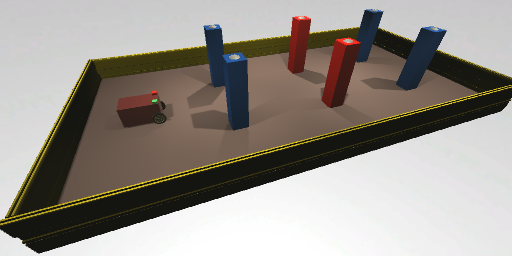
\includegraphics[width=0.3\textwidth]{Bilder/image_printer_images/evaluation_easy.png}}\qquad
    \subfigure[Medium]{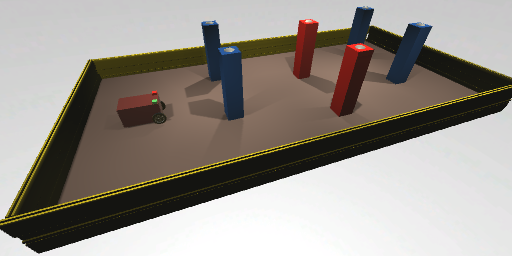
\includegraphics[width=0.3\textwidth]{Bilder/image_printer_images/evaluation_medium.png}}\qquad
    \subfigure[Hard]{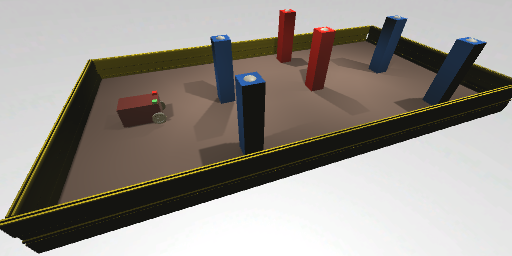
\includegraphics[width=0.3\textwidth]{Bilder/image_printer_images/evaluation_hard.png}}\\
    \caption{Example evaluation tracks for each difficulty setting.}
    \label{fig:track_difficulty_settings}
\end{figure}

\paragraph{Light Setting Description}
There are three light settings for the environment: bright, standard and dark. The different light settings are implemented by varying the light intensities of the arena's light sources and changing the horizon illumination of the agent's camera.

\begin{figure}
    \centering
    \subfigure[Arena Bright]{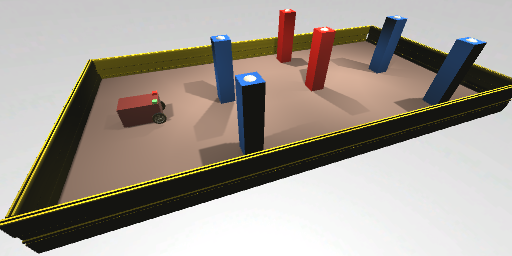
\includegraphics[width=0.3\textwidth]{Bilder/image_printer_images/light_setting_bright_arena.png}}\qquad
    \subfigure[Arena Standard]{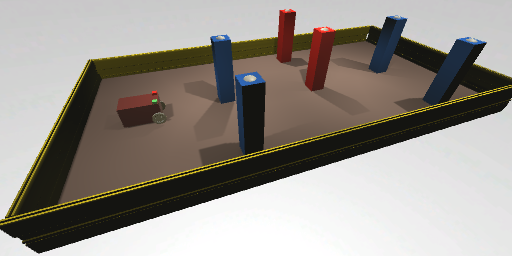
\includegraphics[width=0.3\textwidth]{Bilder/image_printer_images/light_setting_standard_arena.png}}\qquad
    \subfigure[Arena Dark]{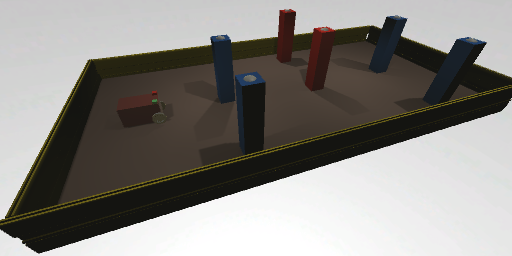
\includegraphics[width=0.3\textwidth]{Bilder/image_printer_images/light_setting_dark_arena.png}}\\
    \subfigure[Agent Bright]{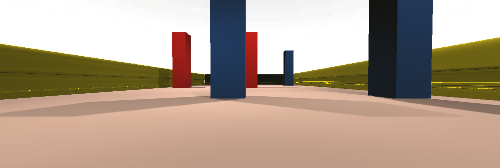
\includegraphics[width=0.3\textwidth]{Bilder/image_printer_images/light_setting_bright_pov_no_preprocessing.png}}\qquad
    \subfigure[Agent Standard]{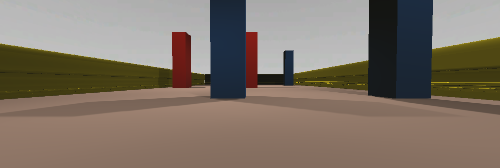
\includegraphics[width=0.3\textwidth]{Bilder/image_printer_images/light_setting_standard_pov_no_preprocessing.png}}\qquad
    \subfigure[Agent Dark]{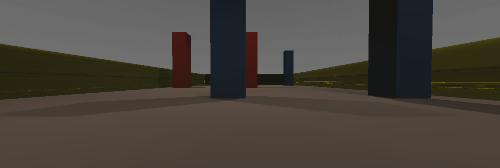
\includegraphics[width=0.3\textwidth]{Bilder/image_printer_images/light_setting_dark_pov_no_preprocessing.png}}\\
    \caption{Arena and agent camera at different light settings.}
    \label{fig:track_light_settings}
\end{figure}

\paragraph{Initial Position of Agent}
The initial position of the agent at the start of an episode is fixed. The starting position is identical for all tracks. The inital orientation is defined by the environment parameter $spawnOrientation$. The parameter specifies the range of rotations around the z-axis.There are three options for the spawnOrientation parameter: Fixed, Random and VeryRandom. For the Fixed option the agent is spawned with an orientation of 0 degrees. In the Random option the agent is spawned with an orientation between -15 and 15 degrees. In the VeryRandom option the agent is spawned with a random orientation between -45 and 45 degrees.

During the training process an orientation from the range is sampled for each episode. In the evaluation process the agent is spawned with unique orientations from the range, see \ref{sec:basic_evaluation_algorithm}.
The ranges for the spawnOrientation parameter influence the difficulty of completing the tracks. Depending on the spawn rotation and the selected track it might not be possible to see the entire first goal from the starting position. This is shown in \ref{fig:spawn_orientation}.


\newcommand{\spawnOrientation}[1]{\includegraphics[width=0.3\textwidth]{Bilder/image_printer_images/#1.png}}
\begin{figure}
    \centering
    \subfigure[Arena $0^{\circ}$ ]{\spawnOrientation{spawnOrientation_Fixed_max}}\qquad
    \subfigure[Arena $15^{\circ}$ ]{\spawnOrientation{spawnOrientation_Random_max}}\qquad
    \subfigure[Arena $45^{\circ}$ ]{\spawnOrientation{spawnOrientation_VeryRandom_max}}\\
    \subfigure[Agent POV $0^{\circ}$]{\spawnOrientation{spawnOrientation_Fixed_max_pov}}\qquad
    \subfigure[Agent POV $15^{\circ}$]{\spawnOrientation{spawnOrientation_Random_max_pov}}\qquad
    \subfigure[Agent POV $45^{\circ}$]{\spawnOrientation{spawnOrientation_VeryRandom_max_pov}}\qquad
    \caption{Example Spawn Orientations and agent camera views for a hard track}
    \label{fig:spawn_orientation}
\end{figure} % the figure shows that the first goal is not always visible from the starting position, very nice


\paragraph{Arena Recording}

Video recordings of episodes can be generated by the unity environment. The episode recordings are created from three different perspectives. The first perspective is the agent's camera view. This video shows the images before preprocessing steps are applied. The second perspective is a top-down view of the arena. The third perspective is a side view of the arena.

Multiple episodes can be simulated in parallel. The video recording is generally not done for all episodes due to performance problems and the large amount of data generated. 
Example videos are shown in the appendix \ref{cha:example_videos}.


\subsection{Agent Description}
\label{cha:agent_description}

The agent is modeled after the NVIDIA JetBot, a small robot designed for educational purposes. The NVIDIA JetBot is equipped with a camera and a differential drive system. The agent's camera is mounted on the JetBot's front and captures the arena from the JetBot's perspective. The camera captures the arena in a 2D image format. In each step the agent receives an action to execute from the Python algorithm. The actions consist of a $leftAcceleration$ and $rightAcceleration$ value. The agent's wheels are controlled using the values for the entire duration of a step. 
The values are in the range of $[-1, 1]$. The agent moves forward when the values are positive. When the right acceleration value is bigger the agent turns to the left and vice versa.


There are two versions of the JetBot agent in the simulation, the DifferentialJetBot and the FourWheelJetBot. The DifferentialJetBot has two driving wheels at the front and a ball supporting it at the back. The DifferentialJetBot applies by different torques to the two front wheels. The two acceleration values are multiplied by a constant factor and applied to the two wheels independently.

The FourWheelJetBot has 2 steering driving wheels at the front and two non-driving wheels in the back. The FourWheelJetBot steers by turning the front wheels in the desired direction. Equal torques are applied to both front wheels. The steering angle is computed from the difference in the two acceleration values. The torque is computed by multiplying the mean of the two acceleration values with a constant factor.

The FourWheelJetBot was used in the work by \textcite{maximilian}. The DifferentialJetBot was developed to match the physical NVIDIA JetBot more closely. The two JetBot designs are shown in figure \ref{fig:jetbots}.


\begin{figure}
    \centering
    \subfigure[Nvidia JetBot Photo]{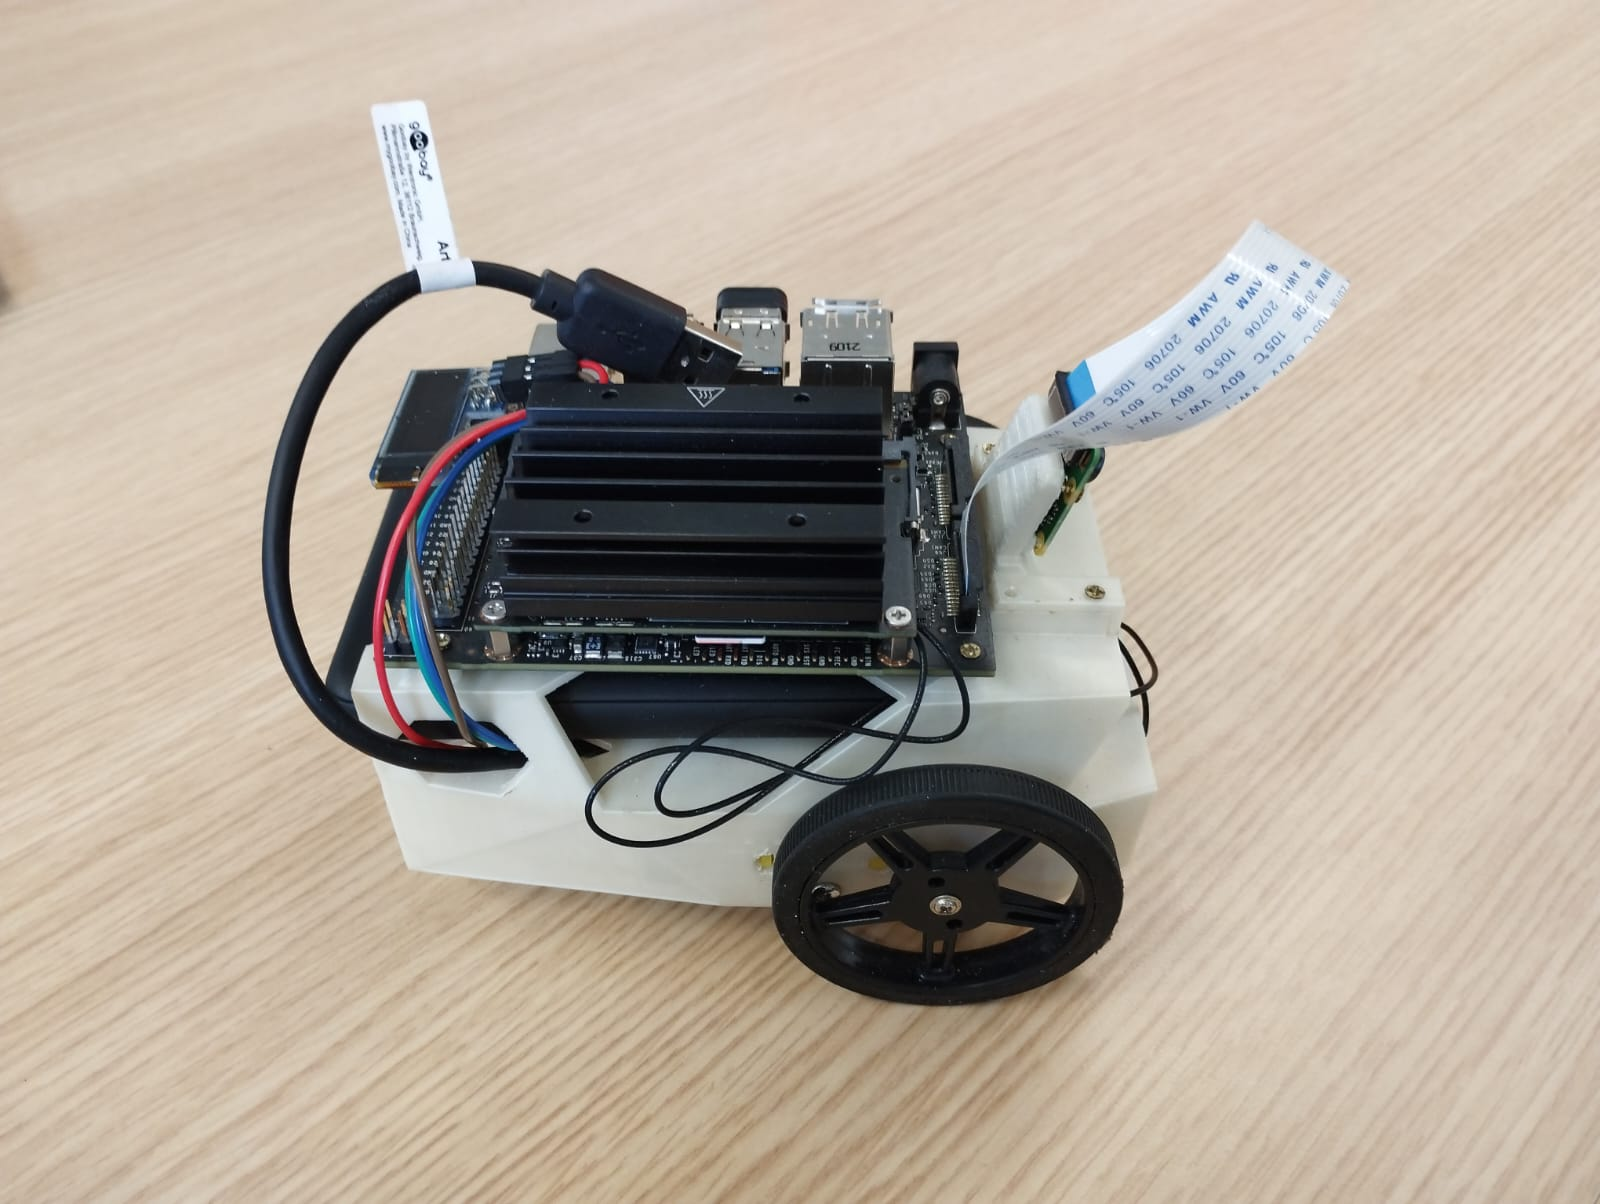
\includegraphics[width=0.3\textwidth]{Bilder/JetBotImages/NvidiaJetBot.jpeg}}\qquad
    \subfigure[DifferentialJetBot]{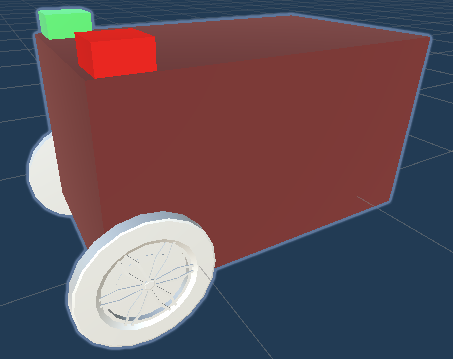
\includegraphics[width=0.3\textwidth]{Bilder/JetBotImages/DifferentialJetBot.PNG}}\qquad
    \subfigure[FourWheelJetBot]{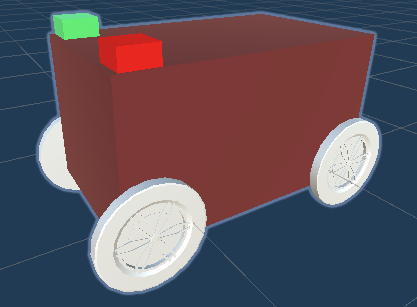
\includegraphics[width=0.3\textwidth]{Bilder/JetBotImages/FourWheelJetBot.PNG}}\qquad
    \caption{Original Nvidia JetBot and simulated JetBot Designs}
    \label{fig:jetbots}
\end{figure}


\subsection{Episode Design}

An episode represents one attempt of the agent at solving a track in the environment. Each episode consists of a series of steps starting from the initial position. Upon episode termination the end status is returned to python. This status is used to compute metrics such as the success\_rate. The agent interacts with the environment in each step. The environment is simulated in Unity during each step. This includes things like agent movement, collision detection and reward calculation.

\subsubsection{Episode Initialization}

The episode initialization prepares the arena. There are five important parameters that define how the episode is initialized. The initialization first generates the obstacles according to the $mapType$ parameter. The $lightSetting$ parameter defines the illumination for the entire episode.
The $jetbotName$ parameter dermines which jetbot version is used \ref{fig:jetbots}. The jetbot is then placed in the arena according to the $spawnOrientation$ parameter.

The $videoFilename$ parameter is used to define the filename for the video recording of the episode. No videos are recorded if this parameter is empty.

The call returns an initial observation to the python algorithm. This observation is used by the agent for the first step.

\subsubsection{Steps}

The agent selects actions to perform in each step. The actions consist of a pair of acceleration values \ref{cha:agent_description}. These values are applied to the agent's wheels for the entire duration of the step. The agent's movement is simulated in the Unity environment for the duration of the step. This results in a new environment state.
The Unity environment calculates the reward obtained during a step. It also registers agent collisions and episode timeouts.


\subsubsection{Step duration}
\label{sec:step_duration}

The duration of each step is defined by the environment settings. There are two destinct modes for the step durations. The first mode is the fixed timestep mode. In this mode the duration of each step is fixed and defined by the environment parameter $fixedTimestepsLength$. The second mode is the variable timestep mode. In this mode each step lasts until the environment receives the next action from the agent.

The fixed step duration mode was used for the training process after experimentation with both modes \ref{sec:step_duration_experiment}. The fixed step duration was set to 0.3 seconds. This allows for precise movements of the agent as the duration is quite short \ref{table:agent_movement_fixed_duration}.

\paragraph{Fixed Duration}

The duration of each step is fixed in this mode. In each step the Unity environment receives an action from the policy. The environment simulation is started and the action is applied to the jetbot agent. The agent moves according to the action and interacts with the environment. The agent collects rewards, collisions and timeouts are detected. The step and environment simulation is terminated when the fixed duration has passed. The duration is defined by $fixedTimestepsLength$ in seconds. The Unity environment then waits until the next step or environment reset. The unity environment does not accept new step commands when the current step is not terminated.
An episode with fixed duration steps is shown in the upper part of figure \ref{fig:unity_timeline_steps_duration}. The figure shows how the Unity environment waits for new steps to start. The figure also shows that the waiting time may not be consistent.

The fixed mode has many advantages. The fixed duration of the steps results in consistency of the step transitions. Given identical step durations and environment state, it is well defined how the agent will move in any step. The environment state after completing a step is well defined.

Furthermore the performance of the policy does not depend on the processing speed of the device. A policy in fixed mode can be transfered to other devices without changing the policy's behaviour. In case of slower policy computation, the unity environment pauses the simulation and waits for the next step command. In case of faster policy computation, the unity environment waits until the current fixed length step is completed before starting the next step.


\paragraph{Variable Duration}

The duration of each step is variable in this mode. The environment simulation is started when the first step is received. In each step the Unity environment receives an action from the policy. The step's action is applied to the jetbot agent. The agent moves according to the action and interacts with the environment. The agent collects rewards, collisions and timeouts are detected. The step is terminated when a new step is received from the policy. The new step is started instantly, there is no waiting time between steps.
The duration of the steps is not fixed, it can change from step to step. It depends on the policy's computation and message transmission time. The environment simulation is not paused during the policy's computation time.
An episode with variable duration steps is shown in the lower part of figure \ref{fig:unity_timeline_steps_duration}. The figure shows how the Unity environment waits only for the first step. The figure also shows that the step sizes may change from step to step.

The biggest advantage and disadvantage this mode is that the step duration depends on the policy's computation and message transmission time. If the policy is computed fast, the average duration of the steps will be shorter. Shorter steps allow for more precise movements. Shorter durations for steps can result in a more capable policy.
A disadvantage is that the step duration can change due to a changed policy computation time. The policy computation time will be different on other devices or when there is additional load on the processing unit.
Changes in step duration might break a trained policy, as the policy has learned to expect a certain environment change for the steps. This environment change might be different for steps with different durations.
Example: The agent might decide to turn right, expecting to be able to stop the turning within 0.2 seconds. If the next step is computed too slow the agent might not be able to stop the turning in time. The agent might then crash into a wall.


% how to build the graphs: https://tex.stackexchange.com/questions/436259/timeline-in-latex
%\definecolor{myLightGray}{RGB}{191,191,191}
%\definecolor{myDarkGray}{RGB}{144,144,144}
%\definecolor{myBlue}{RGB}{0,191,255}
\newcommand\offset{-3}

\begin{figure}[!ht]
    \centering
    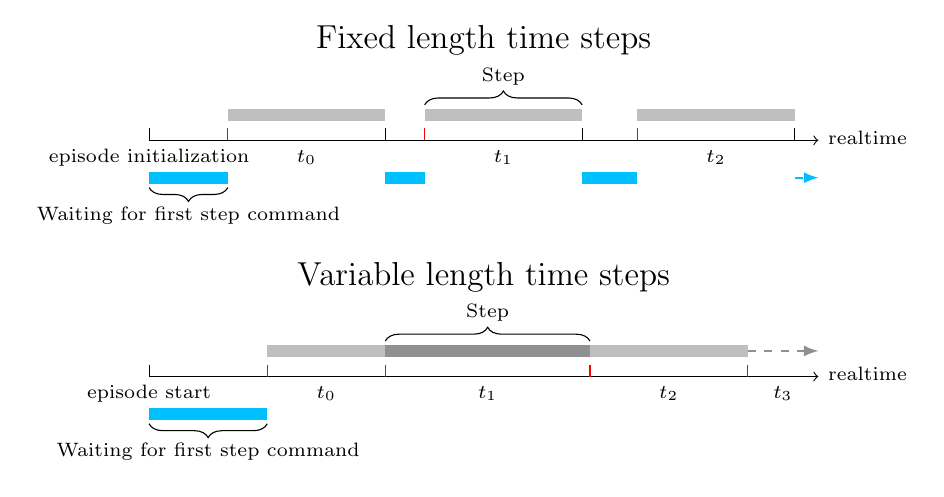
\begin{tikzpicture}[%
            every node/.style={
                    font=\scriptsize,
                    % Better alignment, see https://tex.stackexchange.com/questions/315075
                    text height=1ex,
                    text depth=.25ex,
                },
        ]

        \node[anchor=south] at (4.25,1) {\large Fixed length time steps};

        % draw horizontal line   
        \draw[->] (0,0) -- (8.5,0);

        % draw vertical lines
        % {0,1,3,3.5,5.5,6.2,8.2}
        \foreach \x in {0,3,5.5,8.2}{
                \draw (\x cm,0.15) -- (\x cm,0);
            }
        \foreach \x in {1,3.5,6.2}{
                \draw[red] (\x cm,0.15) -- (\x cm,0); % was 3 pt and 0 pt before
            }
        % displayed fixedTimestepsLength is 2

        % place axis labels
        \node[anchor=north] at (0,0) {episode initialization};
        \node[anchor=north] at (2,0) {$t_0$};
        \node[anchor=north] at (4.5,0) {$t_1$};
        \node[anchor=north] at (7.2,0) {$t_2$};
        \node[anchor=west] at (8.5,0) {realtime};

        % draw scale above

        \fill[myLightGray] (1,0.25) rectangle (3,0.4); % step
        \fill[myLightGray] (3.5,0.25) rectangle (5.5,0.4);
        \fill[myLightGray] (6.2,0.25) rectangle (8.2,0.4);

        \fill[myBlue] (0,-0.4) rectangle (1,-0.55); % wait
        \fill[myBlue] (3,-0.4) rectangle (3.5,-0.55); % wait
        \fill[myBlue] (5.5,-0.4) rectangle (6.2,-0.55); % wait
        \draw[myBlue,dashed,thick,-latex] (8.2,-0.475) -- (8.5,-0.475);

        % draw curly braces and add their labels
        \draw[decorate,decoration={brace,amplitude=5pt}] (3.5,0.45) -- (5.5,0.45)
        node[anchor=south,midway,above=4pt] {Step};
        \draw[decorate,decoration={brace,mirror,amplitude=5pt}] (0,-0.6) -- (1,-0.6)
        node[anchor=north,midway,below=4pt] {Waiting for first step command};

        % second part
        \node[anchor=south] at (4.25, 1 + \offset) {\large Variable length time steps};
        % draw horizontal line   
        \draw[->] (0,\offset) -- (8.5,\offset);

        % draw vertical lines
        % {0,1.5,3,5.6,7.6}
        \foreach \x in {0}{
                \draw (\x cm,0.15 + \offset) -- (\x cm,0 + \offset); % was 3 pt and 0 pt before
            }

        % draw vertical lines for new step commands red
        \foreach \x in {1.5,3,5.6,7.6}{
                \draw[red] (\x cm,0.15 + \offset) -- (\x cm,0 + \offset); % was 3 pt and 0 pt before
            }

        % place axis labels
        \node[anchor=north] at (0,0+ \offset) {episode start};
        \node[anchor=north] at (2.25,0+ \offset) {$t_0$};
        \node[anchor=north] at (4.3,+ \offset) {$t_1$};
        \node[anchor=north] at (6.6,0+ \offset) {$t_2$};
        \node[anchor=north] at (8.05,0+ \offset) {$t_3$};
        \node[anchor=west] at (8.5,0+ \offset) {realtime};

        % draw scale above
        \fill[myLightGray] (1.5,0.25+ \offset) rectangle (3,0.4+ \offset); % step 0
        \fill[myDarkGray] (3,0.25+ \offset) rectangle (5.6,0.4+ \offset);
        \fill[myLightGray] (5.6,0.25+ \offset) rectangle (7.6,0.4+ \offset);
        \draw[myDarkGray,dashed,thick,-latex] (7.6,0.325+ \offset) -- (8.5,0.325+ \offset);

        \fill[myBlue] (0,-0.4+ \offset) rectangle (1.5,-0.55+ \offset); % wait for initial

        % draw curly braces and add their labels
        \draw[decorate,decoration={brace,amplitude=5pt}] (3,0.45 + \offset) -- (5.6,0.45 + \offset)
        node[anchor=south,midway,above=4pt] {Step};
        \draw[decorate,decoration={brace,mirror,amplitude=5pt}] (0,-0.6 + \offset) -- (1.5,-0.6 + \offset)
        node[anchor=north,midway,below=4pt] {Waiting for first step command};
    \end{tikzpicture}
    \begin{tabular}{r@{: }l}
        grey & step, simulation                                    \\
        blue & waiting for step command, no simulation \\
        red  & step command
    \end{tabular}
    \caption{Timeline of steps in Unity for fixed and variable duration}
    \label{fig:unity_timeline_steps_duration}
\end{figure}



\subsubsection{Episode Termination}
\label{time_limit}

The episodes are terminated based on the agent's interactions with the environment. Episodes are always terminated when the agent reaches the finish line or a timeout is reached. Episodes are also terminated when the agent collides with an object and the $collisonMode$ parameter is set to $terminate$.
The timeout is defined by a fixed timelimit of 30 seconds which is increased by further 30 seconds for each passed goal. The timelimit is necessary to terminate episodes where the agent does not reach the finish line. This can be due to the policy's learned behaviour or collisions.

The episode termination status is used by the python algorithms to evaluate the agent performance. The possible termination statuses are:

\paragraph*{Success}

The episode is considered to have been terminated successfully if the agent passed all of the track's goals in order.

\paragraph*{Timeout}

The timeout status is returned when the agent does not reach the finish line within the timelimit and not all goals have been passed successfully.

\paragraph{FinishWithoutAllGoals}

The FinishWithoutAllGoals status is returned when the agent reaches the finish line without passing through all goals.

\paragraph*{Collision}

Collisions of the agent with the goal posts and the arena walls are detected by the environment. The environment parameter $collisionMode$ defines how the agent's collisions are handled. The termination status Collision is returned when the agent collides with an object and the $collisionMode$ parameter is set to $terminate$.




% time-limit, episode termination, step-function, Collisions, rewards

% time limit explain here

% success is now defined as passing all three goals  (without necessarily reaching the finish line)
% this was done as the agent sometimes learns to move back and forth in front of the finish line


\subsection{Reward Function}

The reward function is a function that maps state-action pairs to a scalar reward. These state-action pairs are episode steps. The reward function assigns rewards to each step based on the agent's actions in the environment.

The reinforcement learning algorithm trains the agent to maximise the cumulative reward over an episode. The reward function is a critical component of the reinforcement learning process. It is important to design a reward function that is closely alligned with the goal. The agent could learn unintended behaviour if the reward function is not designed carefully.

\paragraph*{Event Reward}
The goal of the training process is to achieve an agent that traverses the tracks without collisions and passed through the goals in order. The eventReward function describes this behaviour \ref{fig:eventReward_function}. The event reward function is evaluated in each step. A positive reward is awarded to the agent in case it passes a goal or reaches the finish line during the step. A penalty is applied in case the agent misses a goal, collides with an object or the timeout is reached. The magnitude of positive rewards increased was increased compared to the negative rewards. This means that positive events are more important, a single negative event does not cancel out positive rewards.

The maximum amount of reward obtainable from this function per episode is \[num\_goals * goal\_reward + parcour\_reward = 3 * 100 + 100 = 400\]. An agent that maximises the eventReward function will complete the track without collisions. In theory the event Reward should be enough to train an agent that traverses the tracks successfully without collisions.


\begin{figure}
    \centering
    \begin{align}
        EventReward(s_t, a_t) & = \begin{cases}
                                      100,           \text{completed the parcour}           \\
                                      100,             \text{passed a goal}                 \\
                                      -1,            \text{missed a goal}                   \\
                                      -1,            \text{collision with wall or obstacle} \\
                                      -1,            \text{timeout}                         \\
                                      0,             \text{otherwise}                       \\
                                  \end{cases} \nonumber
    \end{align}
    \caption{Event Reward function}
    \begin{tabular}{r@{: }l r@{: }l}
        $s_t$ & state t & $a_t$ & action in state t
    \end{tabular}
    \label{fig:eventReward_function}
\end{figure}


\paragraph*{Dense Reward Functions}
The eventReward function provides the agent with a reward signal that is closely aligned with the desired behaviour. However the eventRewards are only awarded in very few steps. In the optimal episode there are only 4 steps where the reward is non-zero. Three steps where the agent passes a goal and one step where the agent reaches the finish line. The eventReward function is a sparse reward function. Sparse rewards can make it difficult for the agent to learn the desired behaviour. In the case of the eventReward, the agent might never learn to drive towards a goal since there are no rewards that encourage that behaviour. The agent would rely on random exploration alone to discover the positive reward associated with successfully driving through a goal.
Additional reward functions were developed to help the agent learn to complete the tracks. The additional reward functions are dense reward functions. They assign non-zero rewards in most steps. This is comparable to encouraging route following behaviour with a trail of candy versus a big cake at the end of the route.


Dense rewards functions can exasterbate the issue of the agent learning unintended behaviour. Assigning rewards to sub-goal can lead to the agent behaving differently than as indended. The agent might not learn to achieve the overall goal, \textcite{rlbook2020}. This is to be kept in mind when designing and testing the dense reward functions.


\paragraph{Velocity Reward}
The first dense reward function is the velocityReward. It was already developed in previous work \textcite{maximilian} to encourage the agent to drive at full speed. The velocityReward function assigns a reward proportional to the agent's velocity. The reward from driving forward might also help at discovering other rewards, e.g. the positive reward for passing a goal awared by eventReward function.

\paragraph{Orientation Reward}
The second dense reward function is the orientationReward. The orientationReward function assigns a reward based on the agent's orientation. The reward is proportional to the cosine similarity between the agent's orientation and the direction towards the next goal. The orientationReward function encourages the agent to face the next goal. Together with other rewards this can help teach the agent to drive through the next goal.

\paragraph{Distance Reward}
The third and last dense reward function is the distanceReward function. The distanceReward function assigns a reward proportional to the difference in distance between the agent and the next goal. The distanceReward is positive if the agent gets closer to the next goal during a step transition. The distance to the next goal is measured from the midpoint between the two goal posts. The distanceReward function encourages higher driving velocity, as higher velocities result in bigger distance differences and thus rewards. The distanceReward function also encourages the agent to drive strait towards the next goal, as this results in the biggest distance differences. 

In theory the agent should be able to learn to complete the tracks successfully from the distanceReward alone. Maximizing the distance reward would result in the agent driving through all goals in order.

The distance reward is opinionated. It guides the agent towards the midpoint of the next goal. This reward signal may result in a suboptimal path for the agent. The agent might learn to drive through the goal posts at the midpoint. This is not necessary for the desired behaviour. This is a tradeoff that was made when designing the distance reward function.
% opinionated was also discused above at intro of dense reward functions

\paragraph{Composite Reward Function}
The four individual reward functions can be combined in many ways to give the agent dense and meaningful rewards. In previous work the eventReward was combined with the velocityReward to train the agent. In this work we combine the individual reward functions in the composite reward function \ref{fig:reward_functions}. The composite reward function applies scalar weights to the individual reward functions and returns this weighted sum of rewards to the agent. It is crucial to select an appropriate combination of weights for the individual reward functions during training. The weights determine the importance of the individual reward functions and can influence the learned behaviour. If the velocityReward is weighted too high the agent might learn to drive at full speed in circles without ever reaching the finish line. It is also to note that setting a specific reward function's weight to zero essentially removes that reward function.

\begin{figure}
    \centering
    \begin{align}
        R(s_t,a_t)                 & = c_1 \cdot DistanceReward(s_t,a_t) + c_2 \cdot OrientationReward(s_t,a_t) \nonumber \\
                                   & + c_3 \cdot VelocityReward(s_t, a_t) + c_4 \cdot EventReward(s_t, a_t) \nonumber     \\
        DistanceReward(s_t,a_t)    & = \Delta distance(Agent, NextGoalPosition) \cdot \Delta T \nonumber                  \\
        OrientationReward(s_t,a_t) & = S_C(NextGoalPosition - AgentPosition, agentDirection) \cdot \Delta T \nonumber     \\
        VelocityReward(s_t, a_t)   & = v \cdot \Delta T \nonumber                                                         \\
        EventReward(s_t, a_t)      & = \begin{cases}
                                           100,           \text{completed the parcour}           \\
                                           1,             \text{passed a goal}                   \\
                                           -1,            \text{missed a goal}                   \\
                                           -1,            \text{collision with wall or obstacle} \\
                                           -1,            \text{timeout}                         \\
                                           0,             \text{otherwise}                       \\
                                       \end{cases} \nonumber
    \end{align}
    \caption{Complete reward function R with all its components}
    \begin{tabular}{r@{: }l r@{: }l}
        $S_C$ & cosine similarity & $c_i$ & weights           \\
        $s_t$ & state t           & $a_t$ & action in state t
    \end{tabular}
    \label{fig:reward_functions}
\end{figure}
% cosine similarity is one for same direction, zero for orthogonal directions and -1 for opposite directions



\subsection{Collision Mode}

The variable $collisionMode$ describes how the environment handles collisions of the agent with the goal objects and walls. The $collisionMode$ can take 5 different values described in table \ref{fig:collision_modes}. In previous research the episodes were terminated upon collision and when missing a goal \textcite{maximilian}. Furthermore there existed two different training regimes. The first regime trained the agent on the full maps, while the second regime trained the agent on a map with only one goal.

The $collisionMode$ parameter was introduced to allow for more flexibility in the training process and fine control over the event rewards. The inital implementation was the unrestricted mode. Training with the unrestricted mode and event reward showed that the agent's policy started out with extreme negative rewards. The agent quickly learned to avoid these negative rewards by avoiding all collisions and movements. The policy got stuck in a local optimum \ref{fig:event_reward_only_collisionModeUnrestricted_event_reward}.The policy did not learn to complete the parcour during the remainder of training. The unrestricted mode potentially triggers the collision's negative rewards multiple times per step. This results in a big skew of the eventReward function towards negative rewards.

\begin{figure}
    \centering
    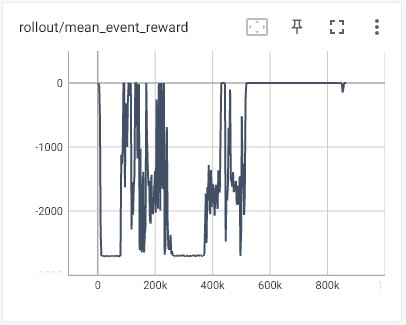
\includegraphics[width=0.3\textwidth]{Bilder/tensorboard_images/eventRewardOnly_collisionModeUnrestricted_eventReward.png}
    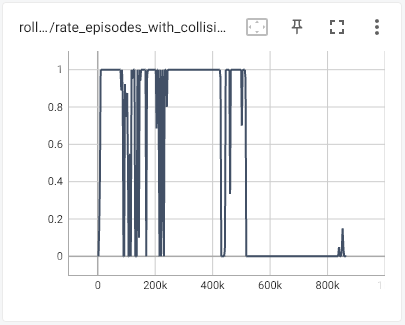
\includegraphics[width=0.3\textwidth]{Bilder/tensorboard_images/eventRewardOnly_collisionModeUnrestricted_collisionRate.png}
    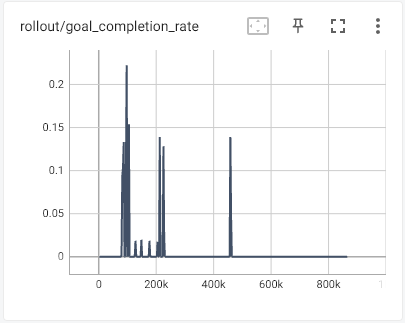
\includegraphics[width=0.3\textwidth]{Bilder/tensorboard_images/eventRewardOnly_collisionModeUnrestricted_goalCompletionRate.png}
    \caption{Event Reward only training with $collisionMode$ $unrestricted$}
    \label{fig:event_reward_only_collisionModeUnrestricted_event_reward}
\end{figure}

The modes $oncePerTimestep$, $oncePerTimestep$, $terminate$ and $ignore$ were introduced to limit the negative rewards caused by collisions. Reducing the negative rewards could lead to a policy that does not avoid collisions and movement as much as. This could lead to more exploration of the environment and a succesful policy.

% maximilian ended the episode on collision and on goal missed https://github.com/Maddi97/master_thesis/blob/main/carsim/Assets/Scripts/CheckpointManager.cs


\begin{figure}

    \begin{center}
        \begin{tabular}{|| p{0.2\linewidth} | p{0.35\linewidth} | p{0.35\linewidth} ||}
            \hline
            collisionMode   & \makecell{Behaviour upon Collision}                                                                                        & Reasoning                                                                                \\ [0.5ex]
            \hline\hline
            unrestricted    & Negative reward is given for each frame with collision.  This can result in multiple penalties given during a single step. & Default behaviour                                                                        \\
            \hline
            oncePerTimestep & Negative reward for collisions is given only once per step.                                                                & Limits the negative reward caused by a collision in a step.                              \\
            \hline
            oncePerEpisode  & Negative reward for collision is only given once  per episode per object.                                                  & Limits the negative reward caused by ongoing collisions.                                 \\
            \hline
            terminate       & Episode is terminated instantly.                                                                                           & No ongoing collisions. The early termination could speed up the neural network training. \\
            \hline
            ignore          & Collisions are ignored, no negative reward is given.                                                                       & The agent might learn to avoid collisions based on other rewards.                        \\
            \hline
        \end{tabular}
    \end{center}
    \caption{Collision Modes}
    \label{fig:collision_modes}
\end{figure}

